\documentclass[12pt]{beamer}

%%%%%%%%%%%%
% Packages %
%%%%%%%%%%%%

\usepackage[english]{babel}
\usepackage{sleek}
\usepackage{tikz}

%%%%%%%%%%%%%%%%
% Bibliography %
%%%%%%%%%%%%%%%%

\addbibresource{references.bib}

%%%%%%%%%%%%%%
% Title-page %
%%%%%%%%%%%%%%

\title{ELEN0016-2 Computer Vision Project: Cell Detection}
\author{Romain Lambermont, Arthur Louis, Tom Navez}
\github{lambi702/CV-Video\_annotation}
\link{https://github.com/lambi702/CV-Video_annotation/}

%%%%%%%%%%%%
% Document %
%%%%%%%%%%%%

\begin{document}
\begin{frame}[t]
\begin{multicols}{3}

\section{Introduction}
Our computer vision project unfolds in two key phases:

\begin{itemize}
  \item \textbf{Background Removal:} Meticulous elimination of backgrounds from original images, a crucial prerequisite.
  \item \textbf{Droplet and Cell Detection:} Our central focus, navigating from background elimination to the presentation of our refined solution.
\end{itemize}

In this presentation, we invite you to explore our methodology, highlighting the challenges and successes encountered during the enhancement of computer vision capabilities in the microscopic domain. 

\section{Creating the Mask}
    \begin{figure}[H]
        \centering
        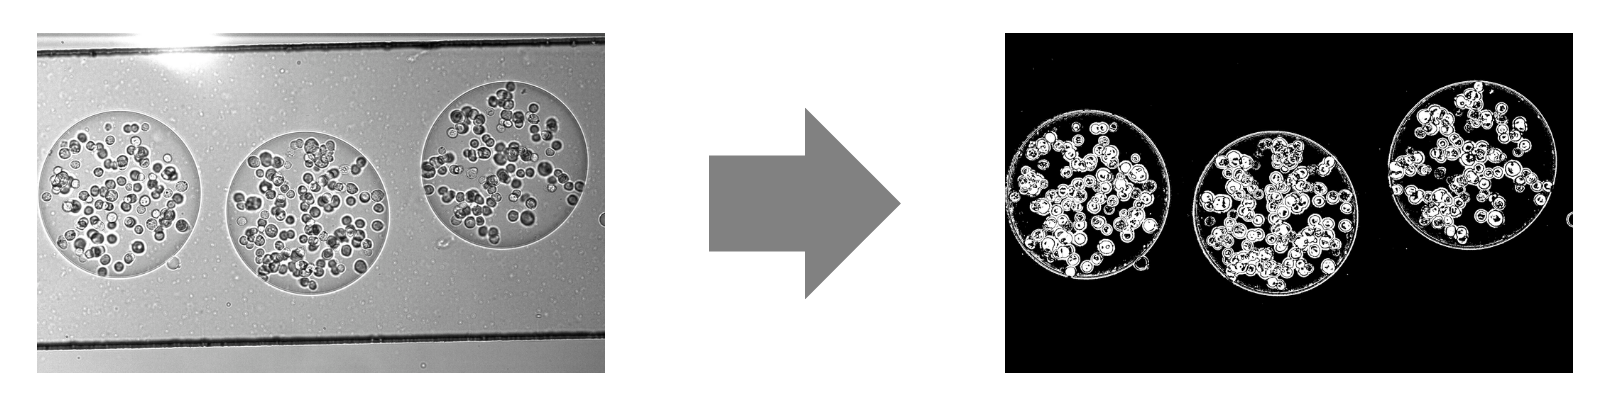
\includegraphics[width=.9\linewidth]{figs/section1.png}
        \caption{Creation of the mask of an example frame.}
        \label{fig:mask}
    \end{figure}

\begin{block}{Mask importance}
 Flawless execution is paramount because any imperfections at this stage introduce noise that persists throughout subsequent steps. Consequently, considerable effort is invested in refining our masking method, extensively testing it across diverse sequences. Addressing exposure variations emerged as a significant challenge in this process.
\end{block}
Initially, we explored an energy score-based method for background reconstruction, but it yielded unsatisfactory results. We then adopted a simpler approach: computing the mean of pixels across 100 frames to establish the background. Subtracting this background from each frame and applying a threshold allowed us to efficiently generate the desired mask.

\section{Isolating the Droplets}
    \begin{figure}[H]
        \centering
        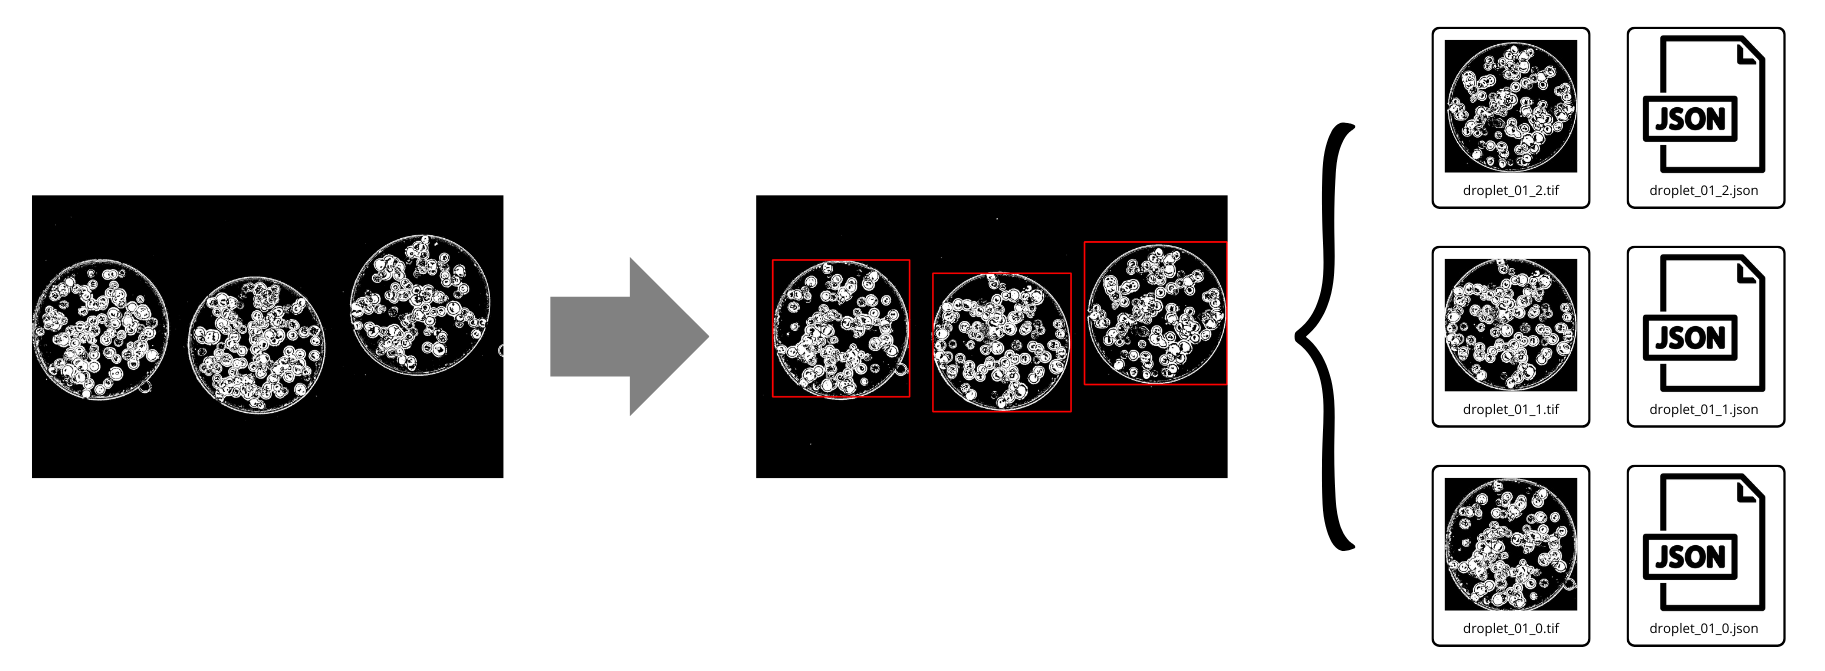
\includegraphics[width=.9\linewidth]{figs/section2.png}
        \caption{Computation of bounding boxes and creation of \texttt{.tif} and \texttt{.json} files for each box.}
        \label{fig:droplets}
    \end{figure}
Bounding boxes were derived from the mask using the Circular Hough Transform function from OpenCV\cite{cv2}. We fine-tuned the function parameters to selectively detect circles within a specific radius range. Subsequently, based on the circle's center and radius, we computed a square around it. Addressing ellipsoidal cells posed a challenge, requiring additional parameter tuning in the function.

\section{Counting and Locating the Cells}
    \begin{figure}[H]
        \centering
        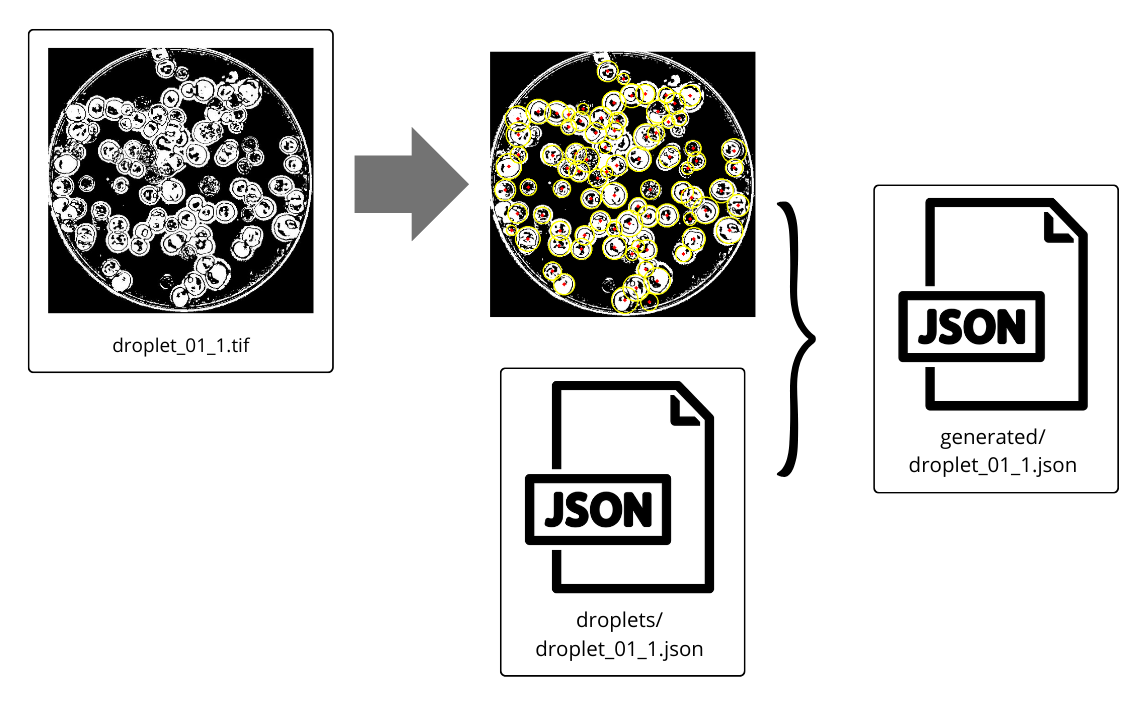
\includegraphics[width=.8\linewidth]{figs/section3.png}
        \caption{Counting and locating the cells inside a zoomed-in droplet and update of the \texttt{.json} file.}
        \label{fig:count}
    \end{figure}

    The method used is the same as before to detect the droplet but on isolated droplet and to a smaller scale.

\vspace{0.25cm}

\begin{alertblock}{Functions used from CV2 \cite{cv2}}
    %% HERE DETAIL THE FUNCTIONS USED IN THE PROJECT
\begin{itemize}
\item findContours:
\begin{itemize}
\item Used between the steps of mask creation and the identification of the bounding boxes.
\end{itemize}
\item HoughCircles:
\begin{itemize}
    \item Task 1: Identifying circles around droplets, further enhancing background removal.
    \item Task 2: Used within isolated droplets to pinpoint cells.
    \end{itemize}
\end{itemize}    
    
    
\end{alertblock}

\section{Combining Data and Sequence Annotation}
    \begin{figure}[H]
        \centering
        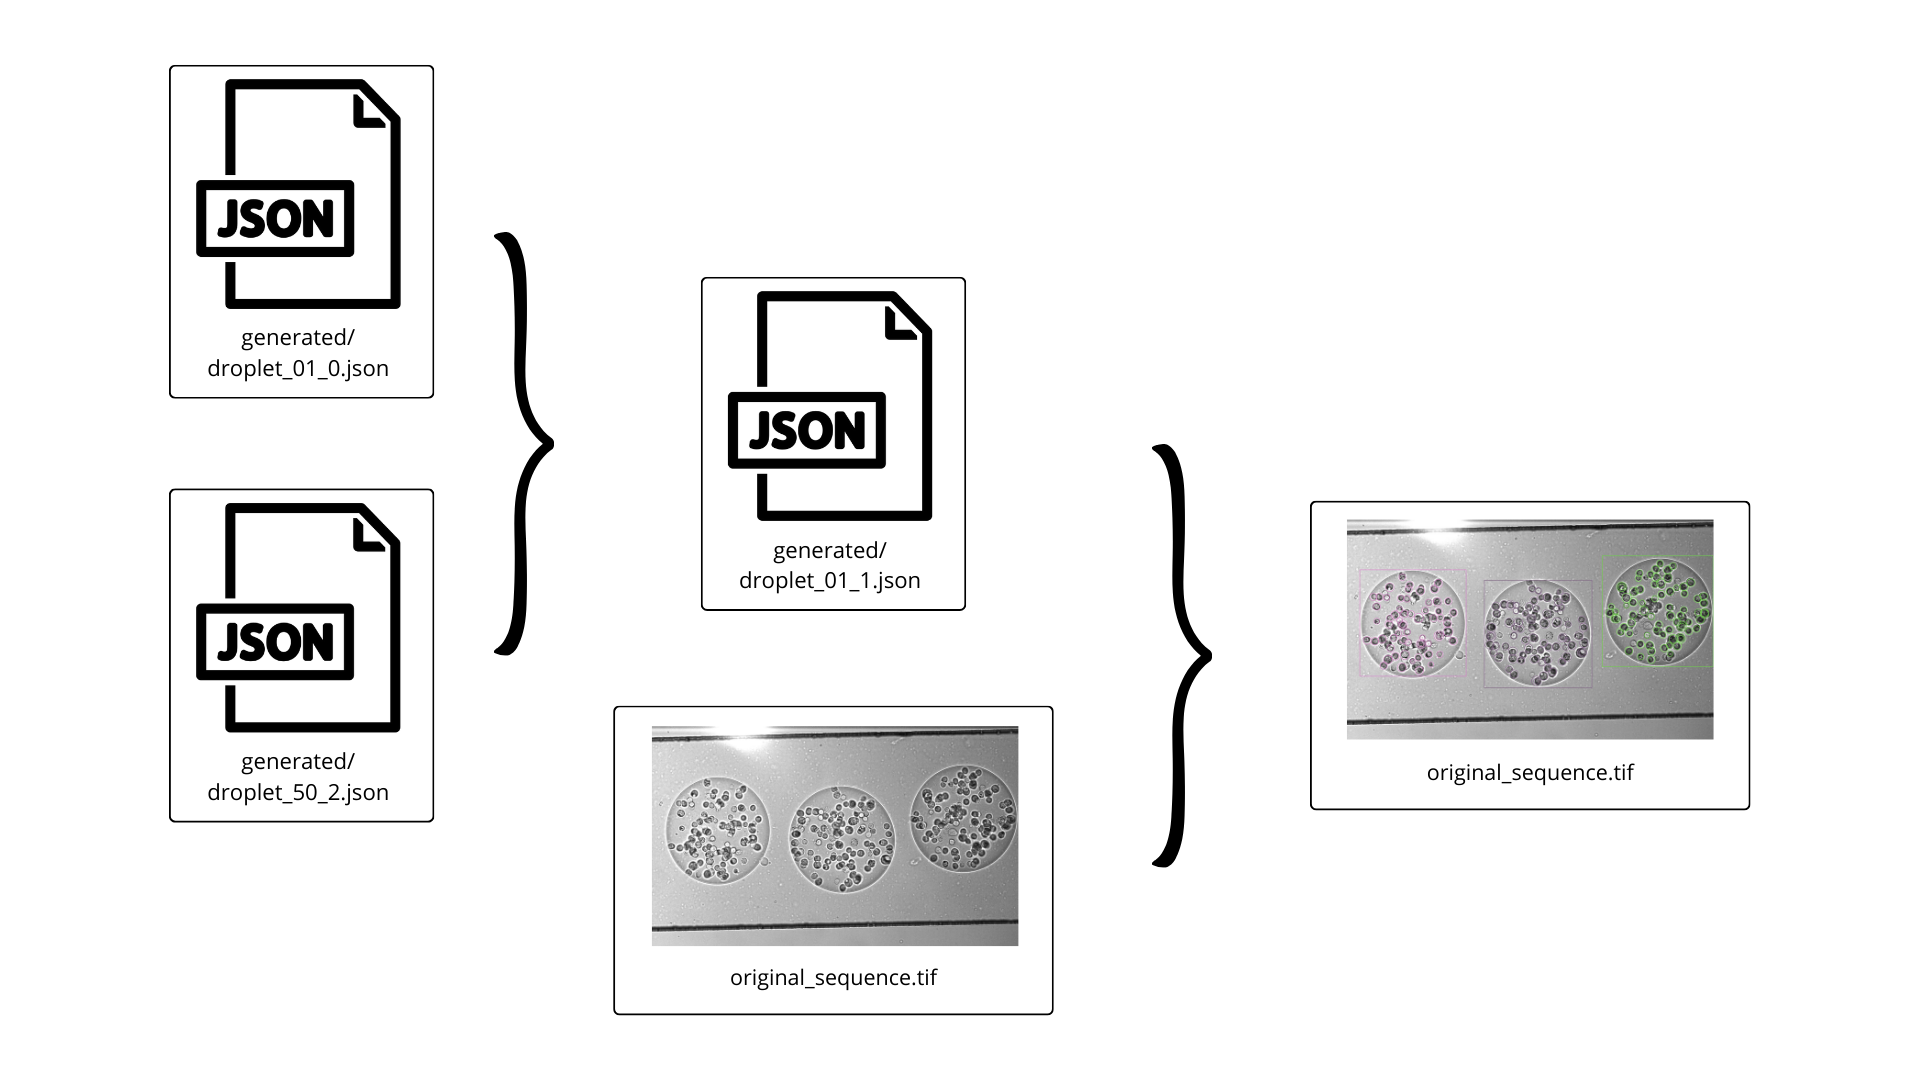
\includegraphics[width=.9\linewidth]{figs/section4.png}
        \caption{Combination of the different \texttt{.json} files and annotation of the original sequence.}
        \label{fig:annotate}
    \end{figure}
\columnbreak 
\section{Statistics}

\begin{table}
    \centering
    \begin{tabular}{l|ccc}
        & \textbf{Mean} & \textbf{std. dev.}\\
        \midrule
        Mask Creation &  $1.66$ s & $\pm35.6$ ms \\
        BB Computation & $6.38$ s & $\pm 145$ ms\\
        Counting Cells & $2$ s& $\pm 64.8$ ms\\
        Sequence Annotation & $50.8$ ms& $\pm 2.81$ ms\\
    \end{tabular}
    \caption{Elapsed time computed over 7 iterations for 30 frames each.}
\end{table}

\section{Alternative Methods and Discussion}

\begin{multicols}{2}
We implemented a Convolutional Neural Network (CNN) on resized, isolated droplets ($448 \times 448$ pixels). Two convolution operations were performed, followed by flattening into a standard fully convolutional network. The flattened image was then concatenated with bounding box coordinates to convey droplet position within the full image.

For loss computation, a blend of Earth Mover's Distance (EMD \cite{emd}) and Mean Squared Error (MSE) for cell count was employed. Regrettably, this approach faced challenges and identified issues:
\begin{enumerate}
\item Loss sensitivity to annotation quality.
\item Network simplicity as a potential limitation.
\item Complexity of Earth Mover's Distance hindering correct usage.
\end{enumerate}
\vfill
\begin{center}
\begin{figure}
    \centering
    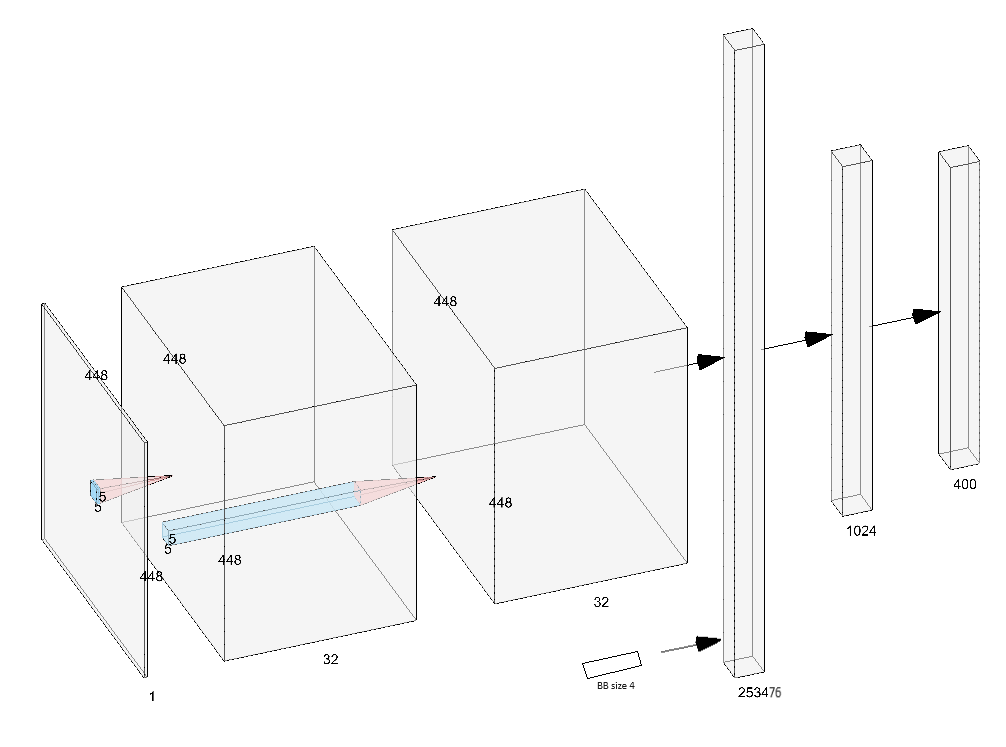
\includegraphics[width=\columnwidth]{figs/nn.png}   
    \caption{Neural Network tried for the project.}
    \label{fig:nn}
\end{figure}
\end{center}

The neural network could have been a better idea if our purpose was only to count the number of cells inside the droplets, but since we also wanted to locate them, we decided to move on and go back to non Deep-Learning based Computer Vision.
\end{multicols}


\section{References}
\printbibliography[heading=none]

\end{multicols}
\end{frame}
\end{document}